\section{Monsterheilung}\label{sec:monster-heilen}
Sobald der Nutzer in den Kampf einsteigt und mit seinen Monstern Angriffe startet, besteht immer die Chance, dass die Monster Leben verlieren und somit nicht die maximale Fähigkeit besitzen, optimal kämpfen zu können. Um die Monster gesund zu halten, wird es dem Nutzer ermöglicht, seine Monster zu heilen.
Die Heilungsmaßnahmen erfolgen bei einer Krankenschwester in einem 'Moncenter'.
\subsection{Mockups}\label{subsec:mockups-monster-heilen}
Jede Krankenschwester befindet sich in einem 'Moncenter' und der Nutzer kann sich jederzeit dorthin begeben.
Wenn der Nutzer einen Dialog mit der Krankenschwester startet, grüßt ihn die Krankenschwester zunächst und fragt ihn, ob er seine Monster wie in Abbildung~\ref{fig: Dialog zwischen Nutzer und Krankenschwester} heilen möchte.
Beim Drücken der Interaktionstaste wird ein Popup wie in Abbildung~\ref{fig: Heilungsfenster} geöffnet, in dem der Nutzer nochmals gefragt wird, ob er seine Monster wirklich heilen möchte.
\begin{figure}[H]
    \centering
    \begin{subfigure}[b]{0.4\textwidth}
        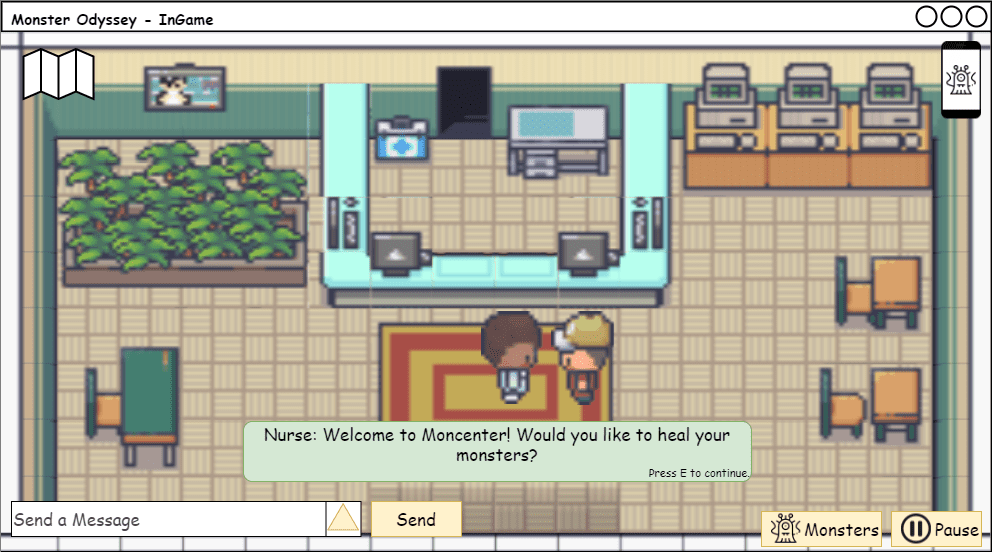
\includegraphics[width=\textwidth]{images/mockups/Heilung/PlayerInMoncenterHealingDialog.png}
        \caption{Dialog zwischen Nutzer und Krankenschwester}
        \label{fig: Dialog zwischen Nutzer und Krankenschwester}
    \end{subfigure}
    \hfill
    \begin{subfigure}[b]{0.4\textwidth}
        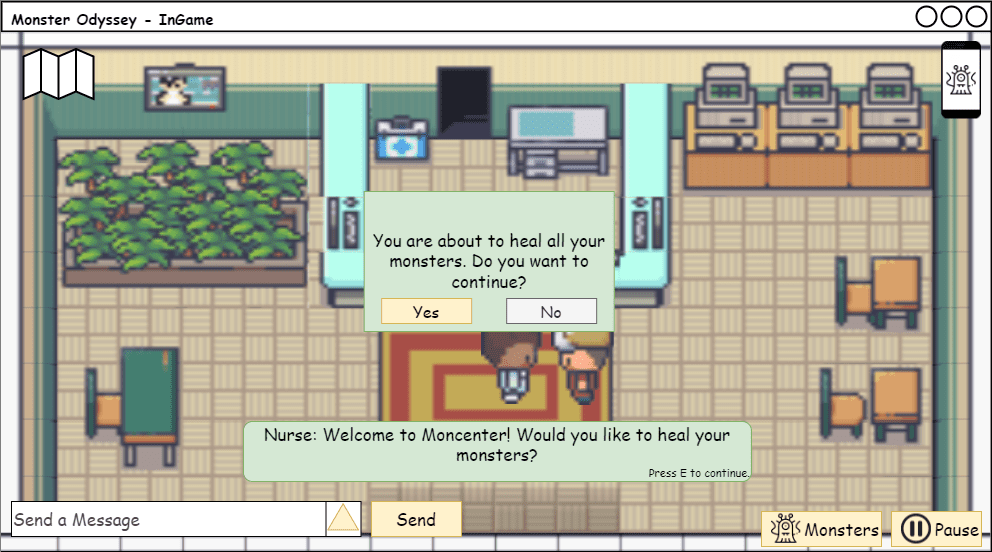
\includegraphics[width=\textwidth]{images/mockups/Heilung/PlayerInMoncenterHealingPopUp.png}
        \caption{Heilungsfenster beim Drücken der Interaktionstaste}
        \label{fig: Heilungsfenster}
    \end{subfigure}
    \caption{Mockup: Interaktion mit Krankenschwester in Moncenter}
    \label{fig: Interaktion mit Krankenschwester in Moncenter}
\end{figure}
Bei dem Pop-up aus der Abbildung~\ref{fig: Heilungsfenster} hat der Nutzer zwei Optionen: die Frage mit „Yes“ oder mit „No“ zu beantworten. Beim Drücken des 'Yes'-Knopfs werden die Monster des Nutzers geheilt und es öffnet sich ein neuer Dialog, in dem die Krankenschwester wie in Abbildung~\ref{fig: Monster geheilt} die Aktion bestätigt. 
Im Gegensatz dazu werden beim Drücken des 'No'-Knopfs die Monster nicht geheilt und die Krankenschwester weist den Nutzer wie in Abbildung~\ref{fig: Monster nicht geheilt} darauf hin, dass er jederzeit wieder in das 'Moncenter' kommen und seine Monster heilen kann.
\begin{figure}[H]
    \centering
    \begin{subfigure}[b]{0.4\textwidth}
        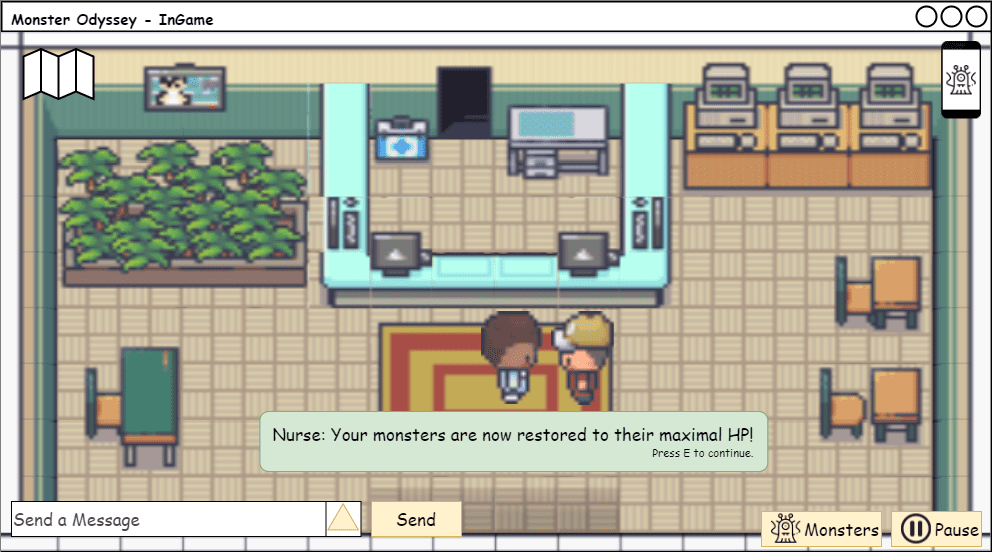
\includegraphics[width=\textwidth]{images/mockups/Heilung/PlayerInMoncenterHealingHealed.png}
        \caption{Monster geheilt}
        \label{fig: Monster geheilt}
    \end{subfigure}
    \hfill
    \begin{subfigure}[b]{0.4\textwidth}
        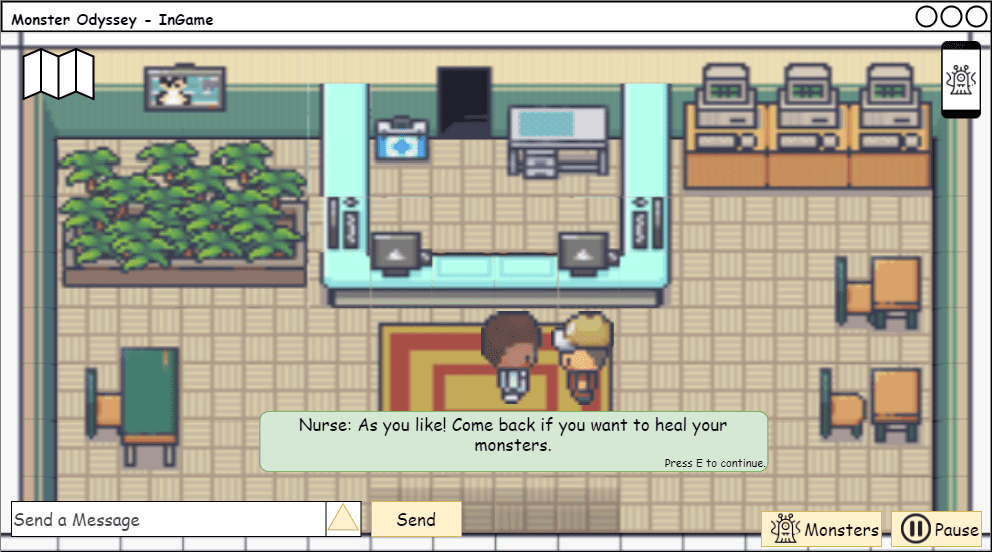
\includegraphics[width=\textwidth]{images/mockups/Heilung/PlayerInMoncenterHealingNotHealed.png}
        \caption{Monster nicht geheilt}
        \label{fig: Monster nicht geheilt}
    \end{subfigure}
    \caption{Mockup: Antwort der Krankenschwester}
    \label{fig: Antwort der Krankenschwester}
\end{figure}
\subsection{Vergleich zwischen Mockups und Implementierung}\label{subsec:vergleich-zwischen-mockups-und-implementierung-monster-heilen}
In der Abbildung~\ref{fig: Vergleich: Dialog zwischen Nutzer und Krankenschwester} ist anzumerken, dass sich die Position der Krankenschwester von dem Mockup unterscheidet. Demzufolge steht die Krankenschwester hinter der Theke in der Abbildung~\ref{fig: Implementierung: Dialog zwischen Nutzer und Krankenschwester}. Darüber hinaus ist ein Unterschied im Dialogtext vorhanden, der aus dem gleichen Grund wie in Abschnitt~\ref{subsec:vergleich-zwischen-mockups-und-implementierung-starter-monster} besteht.
\begin{figure}[H]
    \centering
    \begin{subfigure}[b]{0.4\textwidth}
        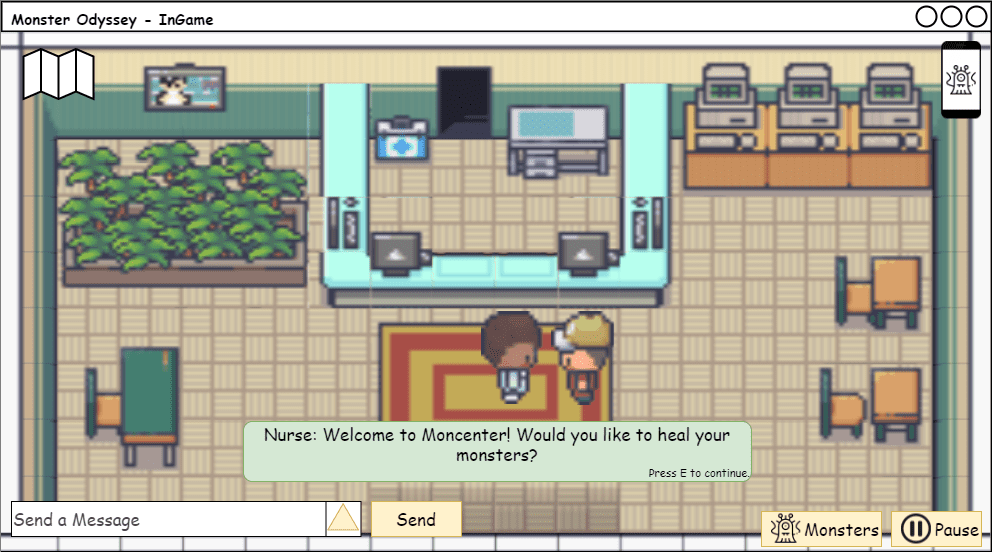
\includegraphics[width=\textwidth]{images/mockups/Heilung/PlayerInMoncenterHealingDialog.png}
        \caption{Mockup: Dialog Nutzer und Krankenschwester}
        \label{fig: Mockup: Dialog zwischen Nutzer und Krankenschwester}
    \end{subfigure}
    \hfill
    \begin{subfigure}[b]{0.4\textwidth}
        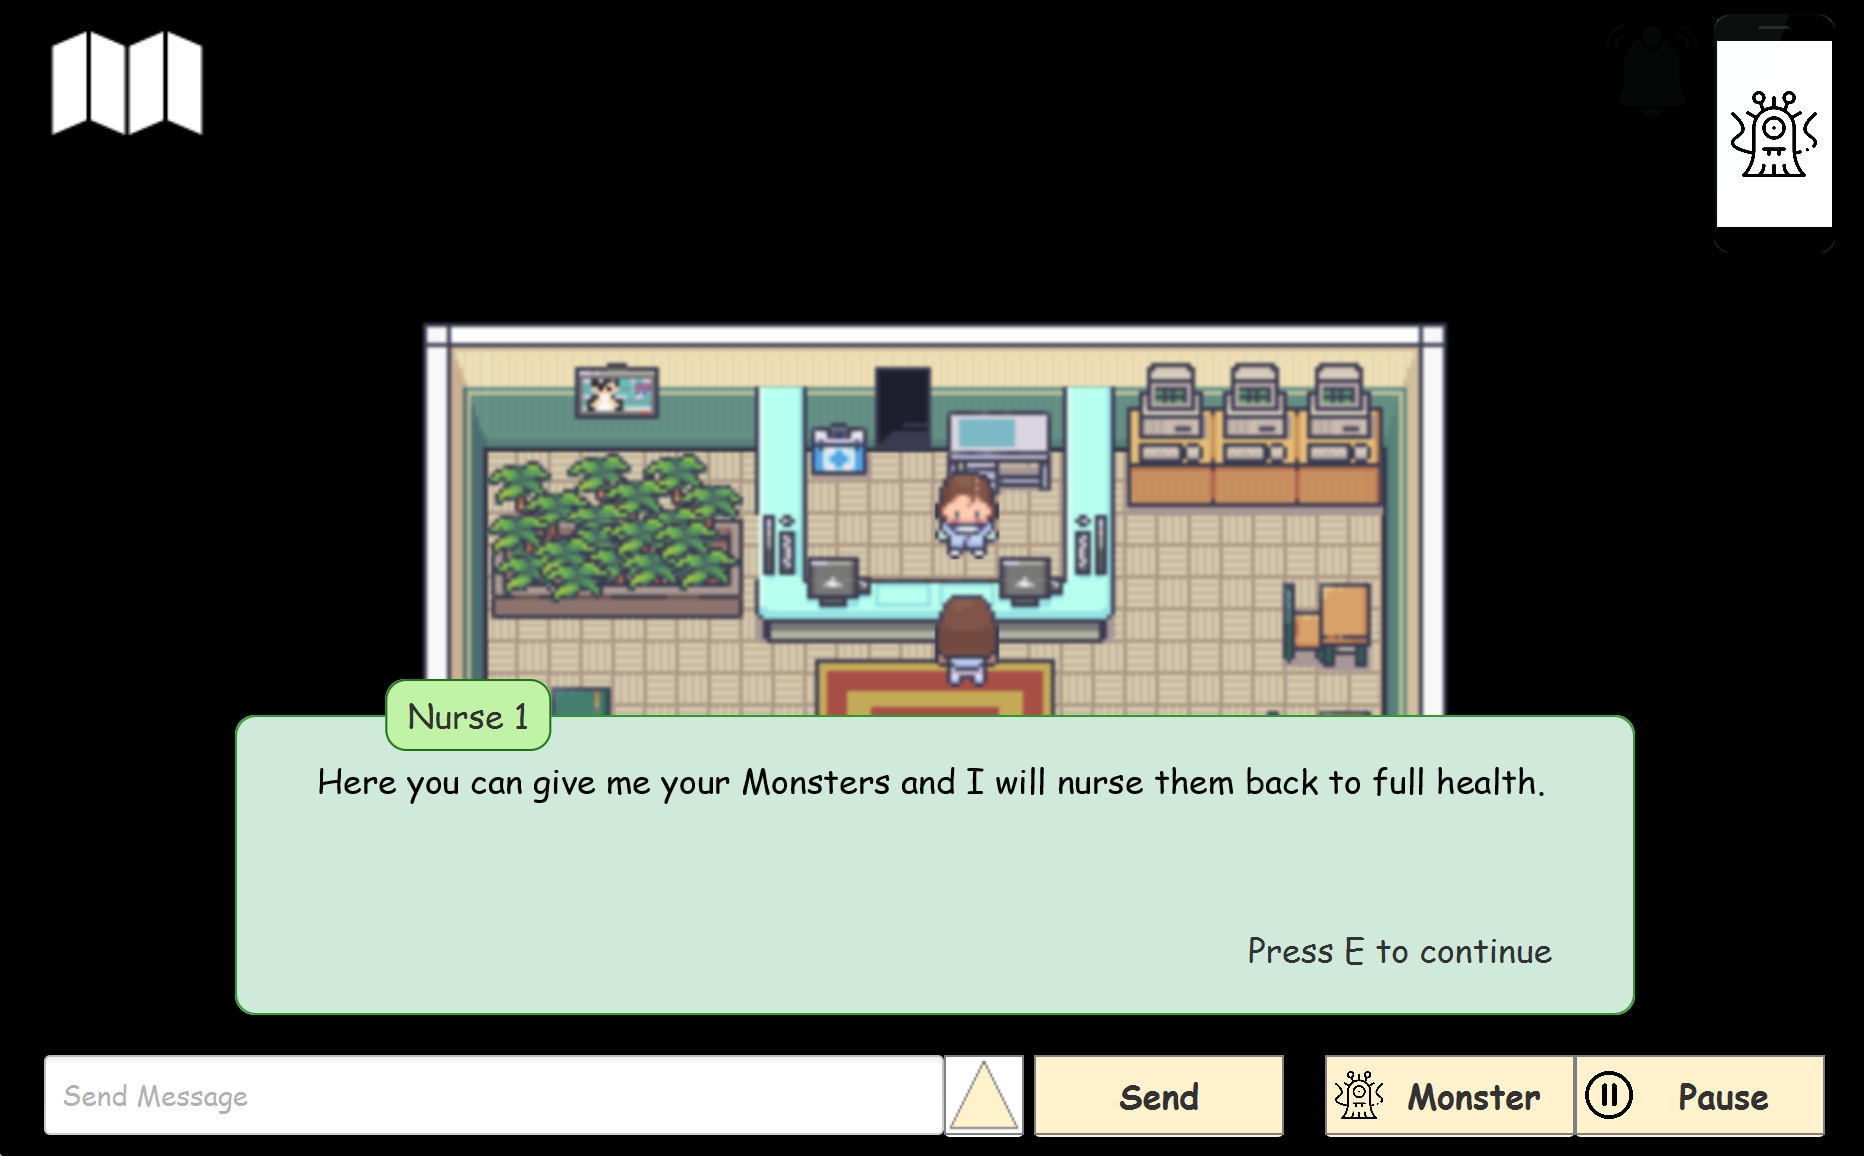
\includegraphics[width=\textwidth]{images/implementation/Heilung/DialogNurseImp.png}
        \caption{Implementierung: Dialog Nutzer und Krankenschwester}
        \label{fig: Implementierung: Dialog zwischen Nutzer und Krankenschwester}
    \end{subfigure}
    \caption{Vergleich: Dialog Nutzer und Krankenschwester}
    \label{fig: Vergleich: Dialog zwischen Nutzer und Krankenschwester}
\end{figure}
Ferner ist aus der Abbildung~\ref{fig: Vergleich: Heilungsfenster} zu erkennen, dass das Popup für das Heilungsfenster aus dem Mockup identisch mit der Implementierung ist, wobei auch hier ein Unschärfeeffekt für den Hintergrund ausgewählt worden ist. 
\begin{figure}[H]
    \centering
    \begin{subfigure}[b]{0.4\textwidth}
        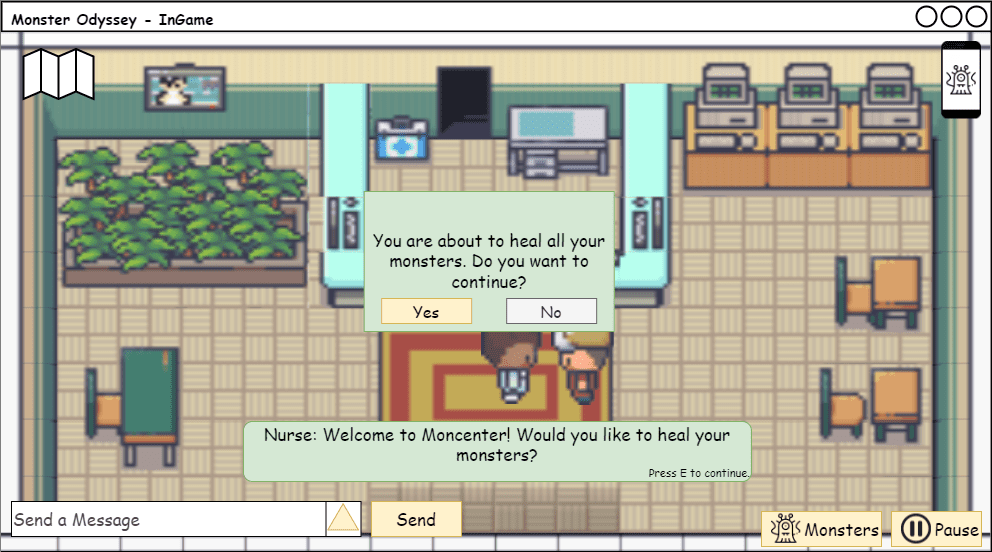
\includegraphics[width=\textwidth]{images/mockups/Heilung/PlayerInMoncenterHealingPopUp.png}
        \caption{Mockup: Heilungsfenster}
        \label{fig: Mockup: Heilungsfenster}
    \end{subfigure}
    \hfill
    \begin{subfigure}[b]{0.4\textwidth}
        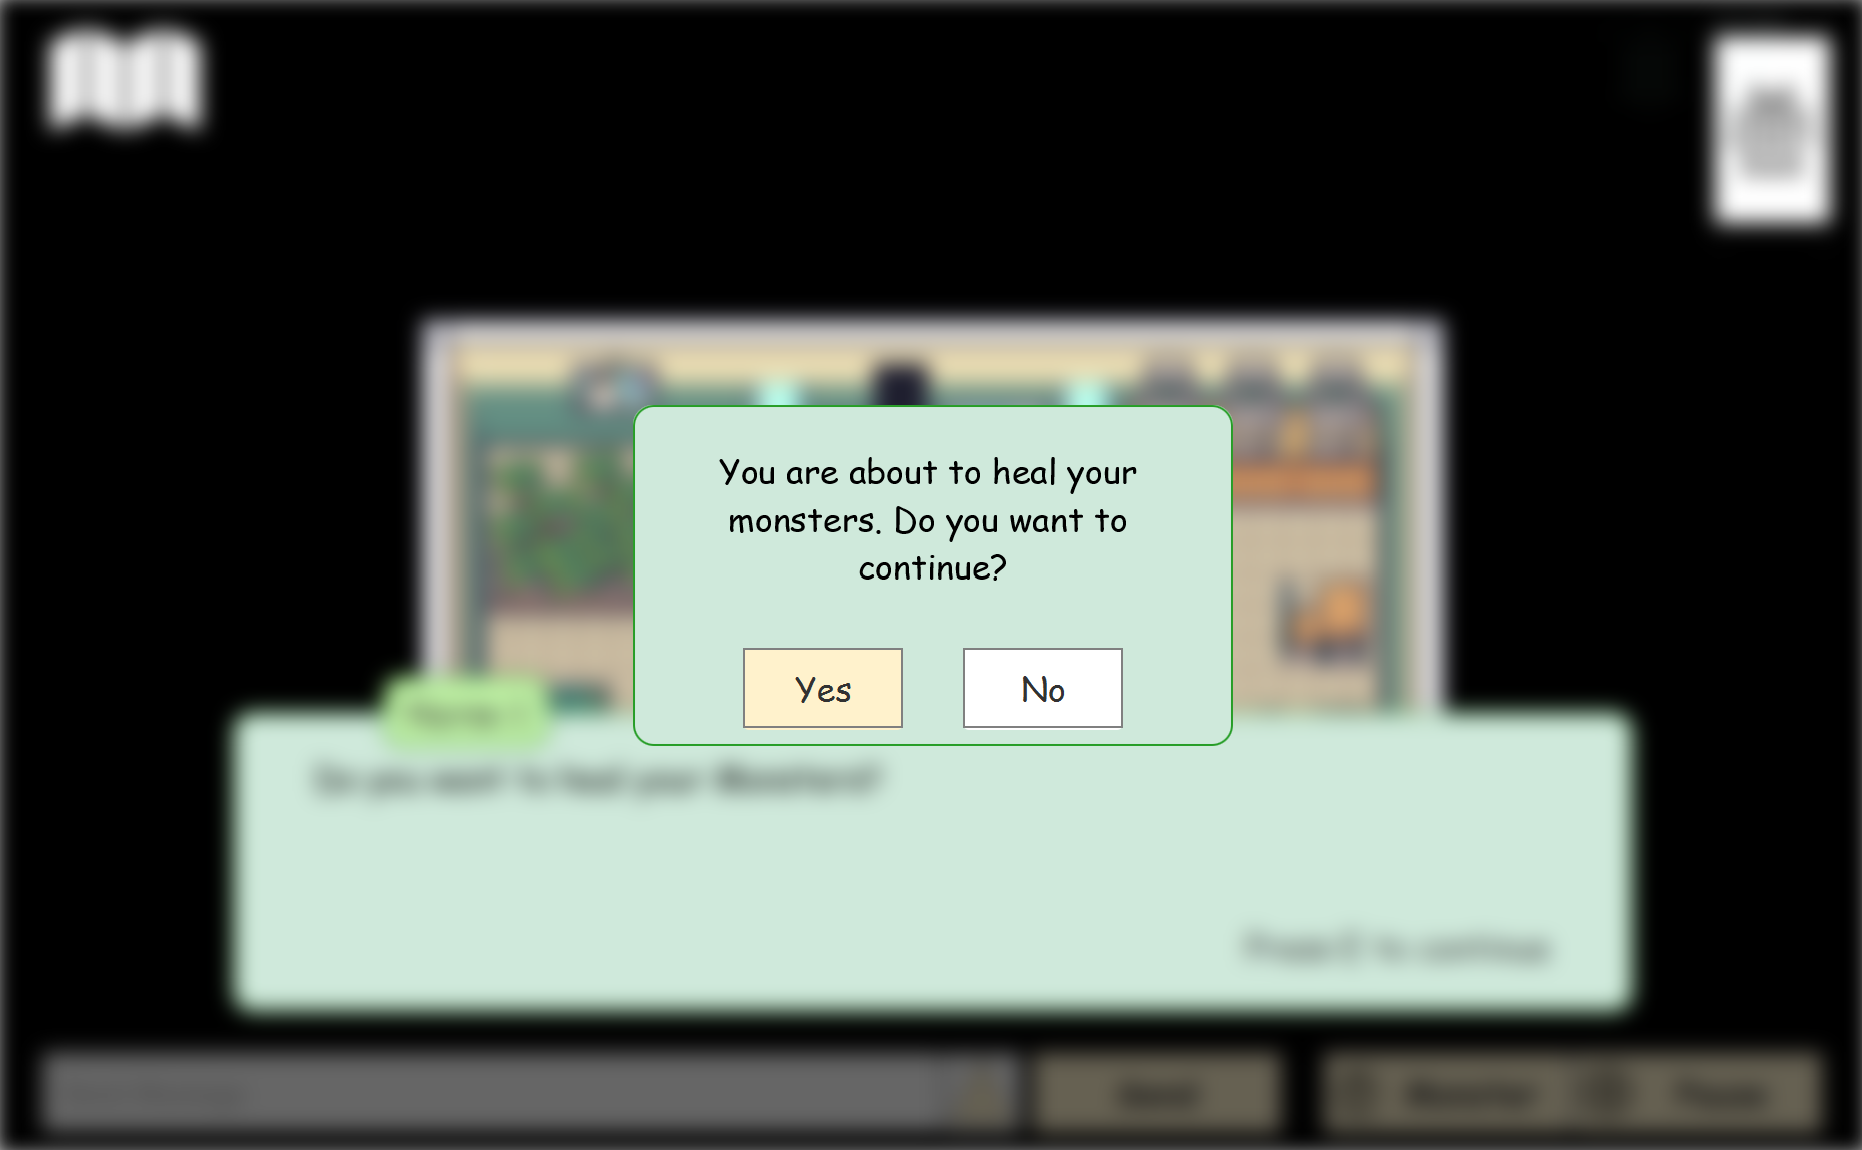
\includegraphics[width=\textwidth]{images/implementation/Heilung/PopupImplementation.png}
        \caption{Implementierung: Heilungsfenster}
        \label{fig: Implementierung: Heilungsfenster}
    \end{subfigure}
    \caption{Vergleich: Heilungsfenster}
    \label{fig: Vergleich: Heilungsfenster}
\end{figure}